\documentclass[10pt,a4paper]{article}

\usepackage[margin=18mm]{geometry}
\usepackage[T1]{fontenc}
\usepackage{lmodern}
\usepackage{microtype}
\usepackage{graphicx}
\usepackage{booktabs}
\usepackage{amsmath}
\usepackage[colorlinks=true,urlcolor=blue!55!black,linkcolor=blue!55!black]{hyperref}
\usepackage{xcolor}
\setlength{\parindent}{0pt}
\setlength{\parskip}{3.5pt}
\setlength{\textfloatsep}{7pt}
\setlength{\intextsep}{7pt}
\setlength{\abovecaptionskip}{4pt}
\setlength{\belowcaptionskip}{2pt}
\renewcommand{\refname}{References}

\begin{document}

\begin{center}
{\Large\bfseries Predicting Concrete Compressive Strength from Mix Design and Curing Age\par}
\vspace{4pt}
{\normalsize Siyu Lu (G2509922G)\par}
\vspace{2pt}
{\small Course: Machine Learning Mini-Project \quad | \quad GitHub: \href{https://github.com/lucylululu721/concrete-strength-ml}{concrete-strength-ml}\par}
\end{center}
\vspace{-7pt}

\section{Problem and Motivation}
Compressive-strength tests take time and destroy the tested specimens. I therefore treated early strength estimation as a supervised regression problem. The inputs are cement, blast-furnace slag, fly ash, water, superplasticizer, coarse aggregate, fine aggregate (all kg/m$^3$), and curing age (days); the output is compressive strength in MPa. Such a model could help screen candidate mixes, although it cannot replace laboratory tests or code checks.

\section{Dataset and Method}
I used the UCI Concrete Compressive Strength dataset: 1,030 observations, eight numerical inputs, one target, and no missing values \cite{uci,yeh}. Using random seed 42, I split it into 720 training, 155 validation, and 155 test observations. The test set was kept aside until model choices had been fixed.

I compared three models. Standardized Ridge regression was the linear baseline. Random forest represented bagging, while gradient boosting added trees sequentially to correct earlier errors. I selected Ridge $\alpha$ from $\{0.01,0.1,1,10,100\}$ and tuned compact grids for the two tree models using validation RMSE. Each selected model was then refitted on the combined training and validation data. Final evaluation used MAE, RMSE, and $R^2$ on the untouched test set. For the validation-selected model, I also calculated permutation importance with 30 repeats. The implementation uses pandas and scikit-learn \cite{sklearn}.

\section{Results and Discussion}
\begin{table}[h]
\centering
\caption{Validation and held-out test performance. Errors are in MPa.}
\label{tab:results}
\small
\begin{tabular}{lrrrr}
\toprule
Model & Val. RMSE & Test MAE & Test RMSE & Test $R^2$ \\
\midrule
Ridge regression & 11.731 & 7.825 & 9.698 & 0.641 \\
Random forest & 5.222 & 3.488 & 4.937 & 0.907 \\
Gradient boosting & \textbf{5.034} & \textbf{2.778} & \textbf{4.161} & \textbf{0.934} \\
\bottomrule
\end{tabular}
\end{table}

Gradient boosting had the lowest validation RMSE, so I chose it before looking at test performance. On the test set it reduced MAE by 64\% and RMSE by 57\% relative to Ridge, and it also improved on the random forest (Table~\ref{tab:results}). Its points follow the one-to-one line more closely, but several high-strength mixes are still underestimated. Permutation importance ranked age and cement highest, followed by water and slag. These rankings describe model sensitivity, not causal effects.

\begin{figure}[h]
\centering
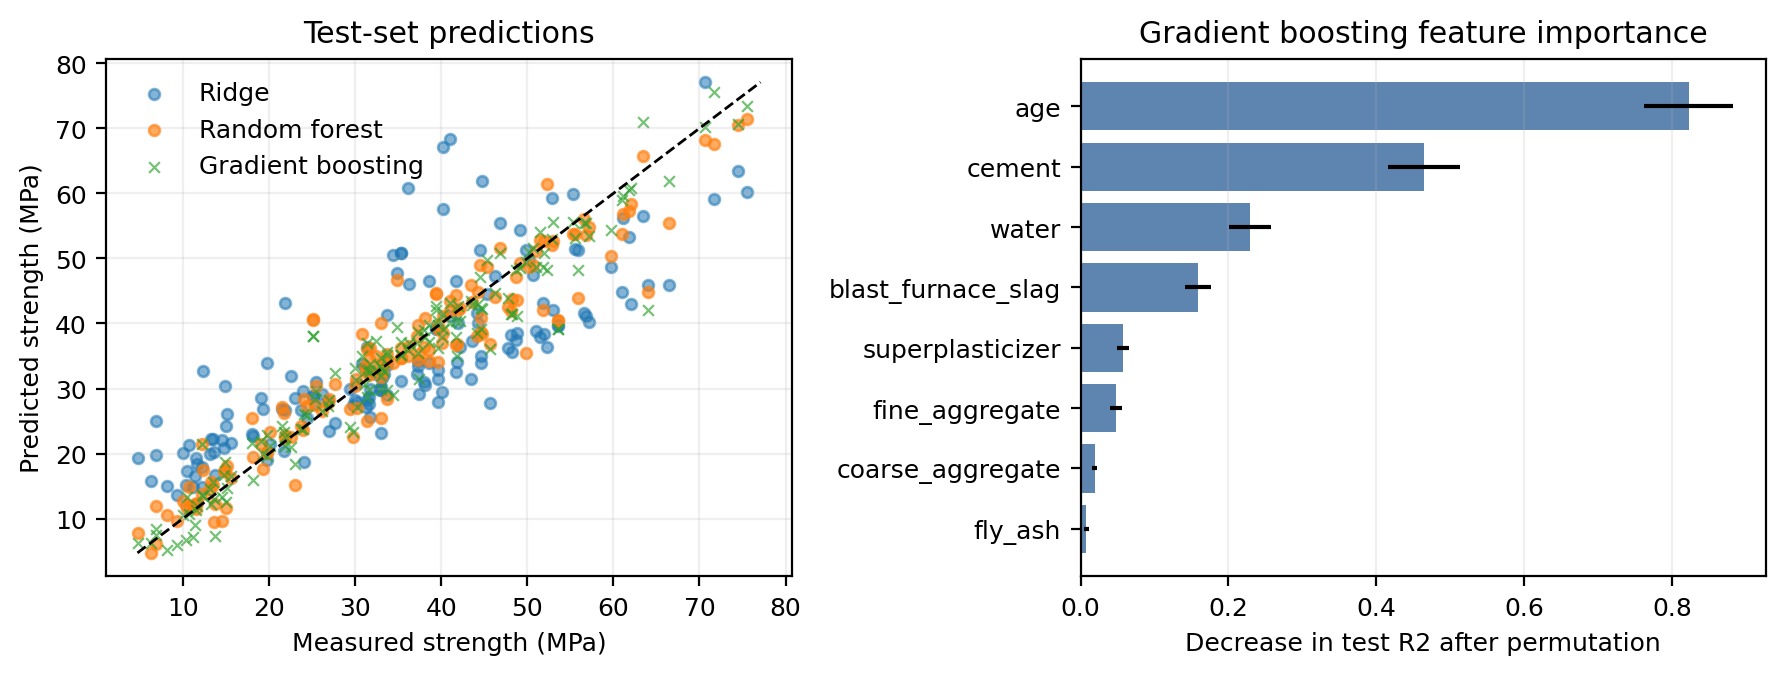
\includegraphics[width=\linewidth,height=5.35cm,keepaspectratio]{images/model_evaluation.png}
\caption{Held-out predictions for all three models and permutation importance for gradient boosting. Error bars show one standard deviation over 30 permutations.}
\label{fig:evaluation}
\end{figure}

\section{Conclusions and Reflection}
Gradient boosting gave the best result, with test MAE 2.78 MPa, RMSE 4.16 MPa, and $R^2=0.934$. The main lesson was that the nonlinear models captured mix interactions that Ridge could not, but a good random-split score is not proof that the model will transfer to a new laboratory. The dataset does not record curing temperature, specimen geometry, testing standard, or material source. A useful next step would be an external or laboratory-grouped test, together with prediction intervals. Until then, the model is suitable for preliminary screening rather than acceptance decisions.

\section*{Reproducibility}
The repository contains the data download and processing code, pinned dependencies, split seed, validation records, tests, and a JSON prediction example. The dataset is CC BY 4.0, and no pretrained model was used.

\begin{thebibliography}{9}\small\setlength{\itemsep}{0pt}
\bibitem{uci} I.-C. Yeh. \emph{Concrete Compressive Strength} [Dataset]. UCI Machine Learning Repository, 1998. \url{https://doi.org/10.24432/C5PK67}.
\bibitem{yeh} I.-C. Yeh. Modeling of strength of high-performance concrete using artificial neural networks. \emph{Cement and Concrete Research}, 28(12):1797--1808, 1998.
\bibitem{sklearn} F. Pedregosa et al. Scikit-learn: Machine learning in Python. \emph{Journal of Machine Learning Research}, 12:2825--2830, 2011.
\end{thebibliography}

\end{document}
